\documentclass[11pt]{beamer}
\usepackage{hyperref}
\usepackage[T1]{fontenc}
\UseRawInputEncoding

\usepackage{graphicx}
\usepackage[utf8]{inputenc}
\usepackage{mathtools}
\usepackage{verbatim}
\usepackage{smartdiagram}
\usepackage{unicode-math}
%\setmathfont{}
\usepackage{comment}
\usepackage{xcolor}
% Cannot enable in Xelatex
\usepackage{pgfpages}
% \setbeameroption{hide notes} % Only slides
% \setbeameroption{show only notes} % Only notes
% \setbeameroption{show notes on second screen}
\usepackage{latexsym,amsmath,xcolor,multicol,booktabs,calligra}
\usepackage{graphicx,listings,stackengine}

\usepackage{tikz}
\usepackage{tikz-feynman}
\usepackage[compat=1.0.0]{tikz-feynman}
%\usepackage{float}

%% Enable only in Xelatex
% \usepackage{pstricks}
\usepackage{feynmp-auto} % or feynmp if you prefer
% Feynman diagrams
%\usepackage{feynmp}
%\usepackage{feynmf}
\DeclareGraphicsRule{*}{mps}{*}{} % for being able to read the produced file

\author{Ana Costa Pereira}
\title{FORM notes}
%\institute [University of Liverpool]{\href{mailto:Ana.Costa-Pereira@liverpool.ac.uk}{\underline{Ana.Costa-Pereira@liverpool.ac.uk}}}
\date{26/06/2026}
\usepackage{QUT}

% defs
\def\cmd#1{\texttt{\color{red}\footnotesize $\backslash$#1}}
\def\env#1{\texttt{\color{blue}\footnotesize #1}}
\definecolor{deepblue}{rgb}{0,0,0.5}
\definecolor{deepred}{rgb}{0.6,0,0}
\definecolor{deepgreen}{rgb}{0,0.5,0}
\definecolor{halfgray}{gray}{0.55}

\lstset{
    basicstyle=\ttfamily\small,
    keywordstyle=\bfseries\color{deepblue},
    emphstyle=\ttfamily\color{deepred},    % Custom highlighting style
    stringstyle=\color{deepgreen},
    numbers=left,
    numberstyle=\small\color{halfgray},
    rulesepcolor=\color{red!20!green!20!blue!20},
    frame=shadowbox,
}

\setbeamercolor{block body alerted}{bg=alerted text.fg!10}
\setbeamercolor{block title alerted}{bg=alerted text.fg!20}
\setbeamercolor{block body}{bg=structure!10}
\setbeamercolor{block title}{bg=structure!20}
\setbeamercolor{block body example}{bg=green!10}
\setbeamercolor{block title example}{bg=green!20}

\begin{document}
%
%
% Capa
%
%
\begin{frame}
    \titlepage
    \begin{figure}[htpb]
        \begin{center}
           
\includegraphics[width=0.35\linewidth]{logo.png}
           
\includegraphics[width=0.35\linewidth]{logo_livinno.jpg}
        \end{center}
    \end{figure}
\end{frame}


\begin{frame}
    \tableofcontents[sectionstyle=show,subsectionstyle=show/shaded/hide,subsubsectionstyle=show/shaded/hide]
\end{frame}










\section{FORM}

\begin{frame}{FORM}
\begin{itemize}
\item Written in C language (some parts C++)
\item Focous on execution speed rather then development speed;
\item Sourced files: header files (declarations), C and C++ files;
\item GUI that allows code folding (including fold nesting);
\end{itemize}
\end{frame}













\section{Sources}

\begin{frame}{FORM sources}
\begin{itemize}
\item each .c or .cc source file there is such a fold and it calls the necessary include files and contains local variables;
\item form3.h contains calls to most of the .h files
\item global variables are contained inside just a few data structs that are defined in the file structs.h
\end{itemize}
\end{frame}












\section{Layout}

\begin{frame}{Layout}
\center
\begin{figure}
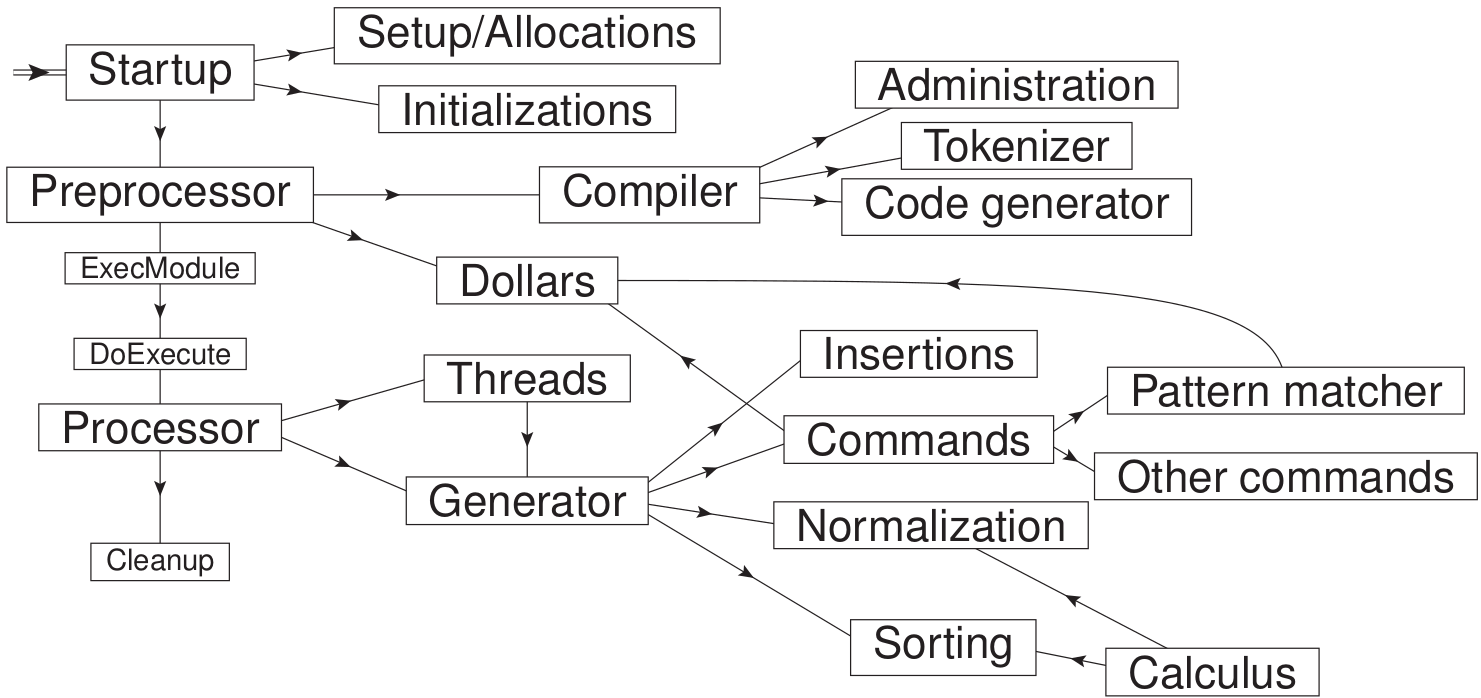
\includegraphics[scale=.2]{form1.png}
\end{figure}
\end{frame}











\section{Expressions and terms}

\begin{frame}
\begin{itemize}
\item \textbf{Expression:} sequence of terms;
\item \textbf{Term:} sequence of numbers of type WORD;
\item Single linear buffer that contains all the terms of the expression and the expression is the sum of all its terms;
\end{itemize}
\end{frame}












\section{Sorting}

\begin{frame}{Sorting}
\begin{itemize}
\item Global variables, buffers and tracking data reside in single master structure A.
\item TFORM runs on multi-core processors POSIX threads (pthreads);
\item If each threads could access and change the glovab memory, it would clash and colapse;
\item Wach threads gets allocated a private copy of A with a pointer, which is $*B$.
\item When compiling for parallel execution, private sub-structures $N$, $R$, $T$ are decoupled from $A$ and placed into teh threads local $*B$;
\item To incorporate FORM and TFORM in the same code source - using Macro AT that gets replaces by the correct option depending on which version the user is running.
\end{itemize}
\end{frame}












\begin{frame}{Sorting}
\begin{itemize}
\item Each worker has a local copy of $*B$ with private data and shared memory;
\item Master makes allocations
\item N workers which get tasks assigned by the master and give the output back to the master once they finish;
\item $N-2$ sortbots that help the sorting
\end{itemize}
\end{frame}









\begin{frame}{Sorting}
\begin{itemize}
    \item Each worker performs a local sort of its generated terms.
    \item Workers produce independent sorted streams.
    \item Sortbots merge pairs of sorted outputs in parallel.
    \item The master performs only the final merge and writes output.
    \item Goal: reduce master-thread bottlenecks and maximize worker utilization.
\end{itemize}

\end{frame}















\begin{frame}{Sorting}
\begin{itemize}
\item Multi-threads: what to do when multiple threads try to update a global variable at the same time?
\item \textbf{Lock routine}: worker has to request a lock both for the reader and the writing and souble check after getting the lock if it wants to update the variable, and only then it can update and the locks are released.
\end{itemize}
\end{frame}












\begin{frame}{Sorting}
\begin{figure}
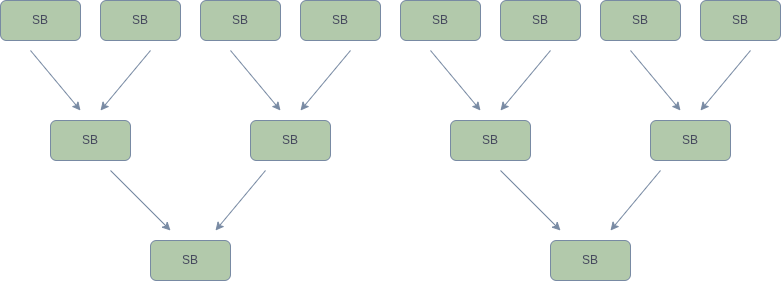
\includegraphics[scale=.35]{images/sortbot.png}
\end{figure}
\begin{itemize}
\item Master makes the allocations for the workers;
\item For each $N$ workers, $N-2$ SB are created; 
\end{itemize}
\end{frame}








\begin{frame}{Sorting}
\begin{itemize}
When a worker runs algebraic expression (example id statement), generated a stream of output terms - there is no rearrengement or combination of terms -  they are packet together on a small buffer one after the other to maximize speed
\\
Various stages in which sorting takes place (once filled up moves to the next):
\item 1 short buffer: routine \textbf{SplitMerge};
\item 2 large buffer (large allocation RAM buffer)
\item 3 sort file (disk spill stage)
\end{itemize}
After we merge results from various cores
\end{frame}








\begin{frame}{Sorting - small buffer}
\begin{itemize}
\item Moving large algebraic terms across the memory is computationally expensive; instead FORM creates an array of memory pointers - each pointer points to a start of a term;
\item \textbf{SplitMerge} evaluated the terms to which the pointers point and sorts the pointers;
\item Identical terms are now consecutively next to each other in memory, where coefficients can combine and cancellations may occur;
\item In the combination of consecutive terms during sorting it may happend that the term that results out of this takes more space in memory compared to the seperate terms before the combination: the tail of the buffer contains a memory pad where this terms are written
\item Once all terms are sorted they are copied to the Large Buffer and the small Buffer is wiped clean to receive the next batch of terms;
\end{itemize}
\end{frame}










\section{TFORM}

\begin{frame}{TFORM}
TFORM code lives mostly in threads.c. Inner workings:
\begin{itemize}
\item Features that deal with the identities of the threads: \textbf{BeginIdentities};
\item Given the number of threads as input, determine how many workers we have;
\item Allocations are made for the workers: \textbf{StartAllThreads};
\end{itemize}
\end{frame}










\begin{frame}{TFORM}
\begin{itemize}
	\item Memory is shared globally between all threads;
	\item Avoid overwritting: each thread makes a private copy of the data: allocation of 1/N of the master's buffer size for each thread and sortbot
    \item After buffers are set up, workers are ready to start working;
    \item Master reads input expressions from the scratch file and distribute terms for workers;
    \item If master sends terms one by one takes too long;
    \item Instead master sends buckets, $1 bucket = 500 terms$ - done by \textbf{ThreadsProcessor};
\end{itemize}
\end{frame}







\begin{frame}{TFORM}
\begin{itemize}
\item Workers receive the buckets by the master and they are finished when the buckets are empty;
\item If a worker is completely done and there are no more buckets to be distributed, the master moves buckets from workers that are still processing terms to these idle workers: \textbf{RunThread};
\end{itemize}
\end{frame}








\begin{frame}{TFORM}
\begin{itemize}
\item After processing the terms, the threads will sort;
\item Each worker has: small buffer, large buffer, sort file, stage4 if necessary;
\item During this final merge we use sortbots -  merge each two workers into a single output, until there is only 2 sortbots left;
\item Then the master merge the final two outputs and writes into the output scratch file
\item Two major bottlenecks in TFORM: reading of the input with division of terms and the inverse tree at the end with the writing to the file by the master;
\item Ways to improve performance: Use \textbf{Brackets} option: all the terms in the bracket will end up in the same worker, so cancellations can be done earlier in the sorting (rather then terms that could cancel ending up in different works and therefore the cancellation would happend only in later stages of the sorting);
\end{itemize}
\end{frame}









\begin{frame}{Best setup for FORM and TFORM}
\begin{itemize}
\item Large memory since disks can slow things down for large expressions;
\end{itemize}
\end{frame}










\begin{comment}


\begin{frame}{Parallel Block Processing \& Overlap Strategy}
    \textbf{Data Fragmentation Strategy:}
    \begin{itemize}
        \item \textbf{Overlapping Blocks:} Raw data streams permit terms to cross block boundaries to maximize ingestion speed.
        \item \textbf{Optimization (Structural Change):} Realizing terms can overlap requires complex boundary tracking. The modern code enforces that \textit{only complete terms} sit inside blocks—rendering historical 0th-block stitching obsolete.
    \end{itemize}

    \vspace{0.3cm}
    \textbf{The "Chained" Locking Mechanism:}
    \begin{itemize}
        \item Threads process blocks sequentially but execute in parallel.
        \item To safely read an overlap boundary, the reading thread must employ a \textbf{Hand-over-Hand (Sliding Window)} lock.
    \end{itemize}
\end{frame}



\begin{frame}{Visualizing Lock \& Release (Hand-over-Hand)}
    \begin{center}
    \small
    \begin{tabular}{rcccl}
        \textbf{Step 1:} & Thread $N$ starts $\rightarrow$ & \color{red}[Lock Thread $N-1$] & \color{red}[Lock Thread $N$] & \textit{(Secures boundary)} \\
        \textbf{Step 2:} & \multicolumn{4}{l}{Thread $N$ safely reads data block and overlapping boundary.} \\
        \textbf{Step 3:} & Thread $N$ finishes $\rightarrow$ & \color{blue}[Release Thread $N-1$] & \color{blue}[Release Thread $N$] & \textit{(Frees next thread)} \\
    \end{tabular}
    \end{center}

    \vspace{0.4cm}
    \textbf{Why this design works:}
    \begin{itemize}
        \item \textbf{No Race Conditions:} Thread $N-1$ cannot destroy or alter its trailing boundary data while Thread $N$ is reading it.
        \item \textbf{Prevents Deadlocks:} Because threads always acquire locks in strict chronological order ($N-1$ then $N$), a deadlock loop is mathematically impossible.
    \end{itemize}
\end{frame}



\end{comment}











\begin{frame}
\textbf{Working of the code:}
\begin{itemize}
\item Terms are allowed to overlap between blocks;
\item Reading thread always locks pair of locks - the current thread and the previous thread;
\item 0th block - the overlap in the end of term is copied to 0th so that the terms are contiguous - this is no longer needed when we impose that only full terms can fit into the blocks
\end{itemize}
\end{frame}










\begin{frame}
Before changes
\begin{itemize}
\item Default buffer sizes were increased over time 
\item Size of sortbots increased;
\item The output from a worker fits in a single block $\longrightarrow$ no advantage on running in parallel;
\item Each stage of sortbot merge tree runs one after the other
\item Terms can be partially shared between blocks: when a term is being written in a block and the block finishes, the term keeps being written into the next block
\end{itemize}
\end{frame}













\begin{frame}
After changes
\begin{itemize}
\item Blocks are made smaller
\item Whole terms can only be written in one block: if it does not fit, it goes into the next block
\item Workers that fill the blocks try to detect if there is a reader waiting for them
\item Obtain a lock of the block before filling the block; if not, it means the reading thread already has the lock which means that it is processing the block which means it wants small terms from the current filling block, so we move on to the next block in writing thread
\item There is always a minimum number of terms in the block - MINIMUMNUMBEROFTERMS
\end{itemize}
\end{frame}

















\begin{frame}
Some results after the changes
\begin{itemize}
\item No decrease in performance for any tests;
\item Performance improvement for benchmarks where term merging is expensive (PolyRatFun, PolyRatFunExpand)
\item Forcer, mbox1l
\end{itemize}
\end{frame}



















\end{document}
